\documentclass{article}
\usepackage[utf8]{inputenc}
\usepackage[czech]{babel}
\usepackage{graphicx}

\title{Raketka - uživatelská dokumentace}
\author{Kateřina Nevolová \\ \texttt{katka.nevolova@gmail.com} \\ I-Y-40, 73502469}

\begin{document}
\maketitle

Raketka je jednoduchá hra pro jednoho hráče simulující vesmírný souboj
nepřátelských bitevních lodí. Hráč ovládá poslední výplod pozemské civilizační
technologie a navádí jej proti nekonečným hordám nepřátel z SM (Svazu
Mimozemšťanů). Obě strany samozřejmě ovládají pokročilé zbraňové systémy.

\section{Ovládání}

Program se spouští z terminálu příkazem 
\texttt{./raketka}

Po spuštění programu okamžitě začíná hra. Raketku vesmírem navádíme pomocí
kurzorových šipek, střelba je poté vedena mezerníkem. Ze hry je kdykoliv možné
odejít klávesou escape.

\section{Herní systém}

Jednotky na hráče útočí ve vlnách, složených z několika druhů nepřátel. Hlavní
vlnu tvoří formace obyčejných plavidel jejichž obranu zajišťují pomalé, ale
velmi odolné vesmírné tanky. Poslední nepříjemnou jednotkou je rychlý a střely metající berserker.

Vesmírný souboj je ozvláštněn všemožnými power-upy, občasně padajícími ze
sestřelených nepřátel. Modrý bonus zajistí dvacetivteřinový neprolomitelný
štít. Po sebrání zeleného bonusu se, na stejnou dobu, stane z děla raketky
nezkrotný kulomet. Žlutý buff přidá hráči jeden život (power level). Bílý bonus
přidá namalé skóre. 

Po destrukci jedné vlny nepřátel hra postoupí do dalšího kola, hráč přitom
získá nový power level a s ním i možnost rychlejší střelby. Naopak hráč
power ztrácí pokud je čímkoliv zasažen, pokud tímto klesne jeho power na nulu,
hra končí.

\section{Screenshoty}
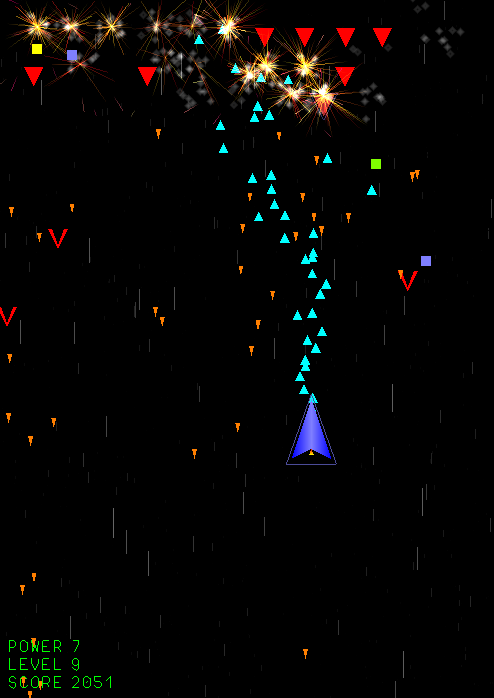
\includegraphics[width=4cm,height=5.6cm]{combat.png}
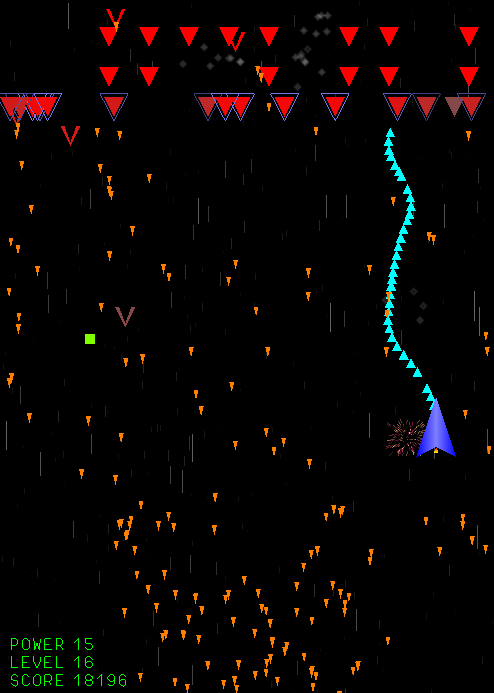
\includegraphics[width=4cm,height=5.6cm]{being_hit.png}
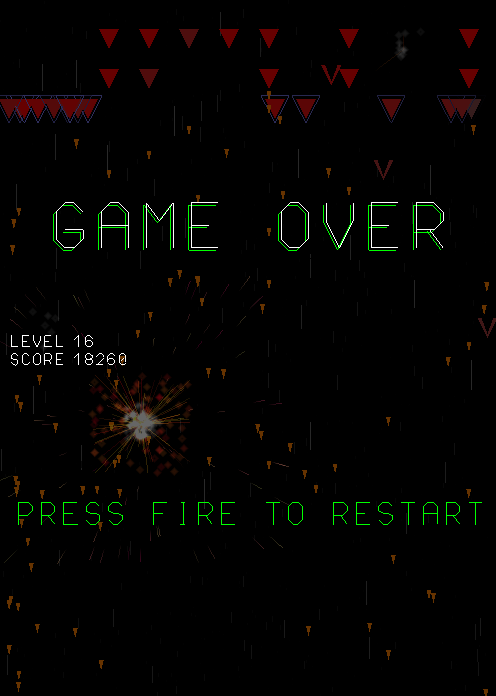
\includegraphics[width=4cm,height=5.6cm]{game_over.png}

\end{document}

